\section{Setting}

\subsection{Evaluation Metrics}

The two main measurements for the performance of our new architecture are learning efficiency and transfer learning capability.
The learning efficiencies are measured in two different ways. First, the performance ILP(RL) is compared with exisitng RL algorithms in terms of
convergence rate, which is measured in terms of number of episodes that the agent needs to get to an optimal policy.
Second, the convergence of learning by ILASP is measured in terms of the number of hypothesis improvement devided by the total number of hypothesis improvement at episode 0.
The reason we are measuring it at only episode 0 is that empirically the agent learns the target hypothesis at episode 0 and there is no hypothesis refinement after episode 0.
This gives a normalised convergence rate of ILASP learning with the maximum 1.

\subsection{Benchmark}
We use two existing RL methods as benchmarks: Q-learning and tile-coding.
Q-learning is widely used RL technique, and given the environments used for the experiments are discrete and deterministic, this method is sufficient enought for our experiment.

Another benchmark is tile coding, which is a type of linear function approximation techniques described in Chapter XX.
The reason for using an extra benchmark is that the comparision with q-learning might not be a fair comparision,
since ILP(RL) has one extra assumption: the agent knows surrounding information (whether there are walls in adjacent cells),
which is not a common assumption for Q-learning. Thus we incorporate the same surrounding information as features, and update the weights of each feature as a learning.
We compare the performance of ILP(RL) with these two methods.

\subsection{Parameters}
\begin{table}[!ht!b]
\centering
\begin{tabular}{lll}
\hline
Parameter            & ILP(RL)    & Benchmarks      \\ \hline
The number of episode& 100        & 100        \\
Time steps per episode& 250        & 250        \\
The number of experiments& 30       & 30       \\
% Discount rate        & 0,5       & 1.4e-2       \\
Alpha                & N/A       & 0.5       \\
Epsilon              & 0.4        & 0.1        \\
\end{tabular}
\caption{Parameters used in the experiments}
\label{param}
\end{table}

All the matrices used in the experiments are summarised in Table \ref{param}.
Epsilon for ILP(RL) should be higher, since the agent follows the generated plan,
whereas benchmark algorithms update value function with the degree of alpha.
We conducted several experiments using different environments to highlight each aspect of the algorithm.

Since the performance of the agent is affected by the randomness of the exploration,
and ILP(RL) is highly dependent on how quickly the agent finds the goal,
each experiment is conducted 30 times and the perform is averaged across the experiments.
At each episode, we also measure the performance without exploration to see the pure optimal policy.

\section{Experiment Results}
\label{learning_evaluation}

\subsection{Experiment1}
\begin{figure}[!htb]
\centering
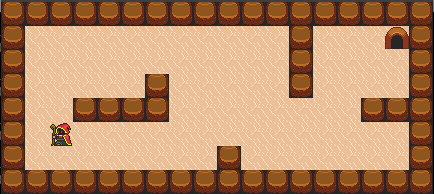
\includegraphics[width=0.5\textwidth]{./figures/experiment1}
\caption{Enviroment for experiment 1}
\label{experiment1}
\end{figure}

The purpose of the first experiment is how the algorithm learns the model of the environment, or hypothesis in ILASP.
The environment are defined as a simple maze where the goal is located the right uppper corner as shown in Figure \ref{experiment1}.

The shortest path is taking the lower path instead of the upper one.

\begin{figure}[!htb]
\centering
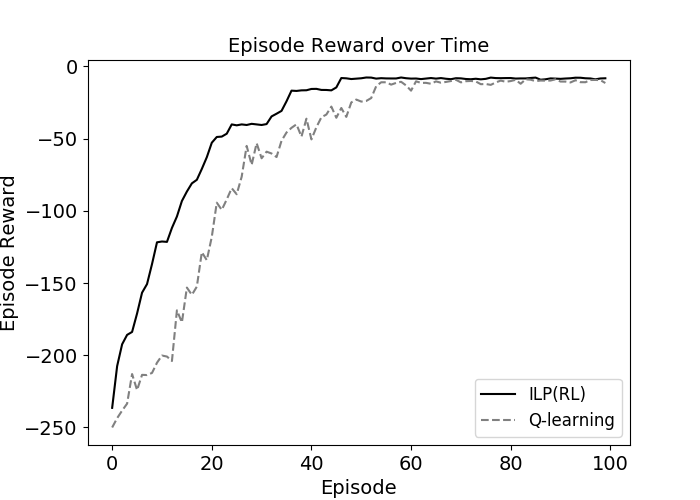
\includegraphics[width=1.0\textwidth]{./figures/experiment1_training}
\caption{Experiment 1 results of training performance}
\label{experiment1_training}
\end{figure}
\begin{figure}[!htb]
\centering
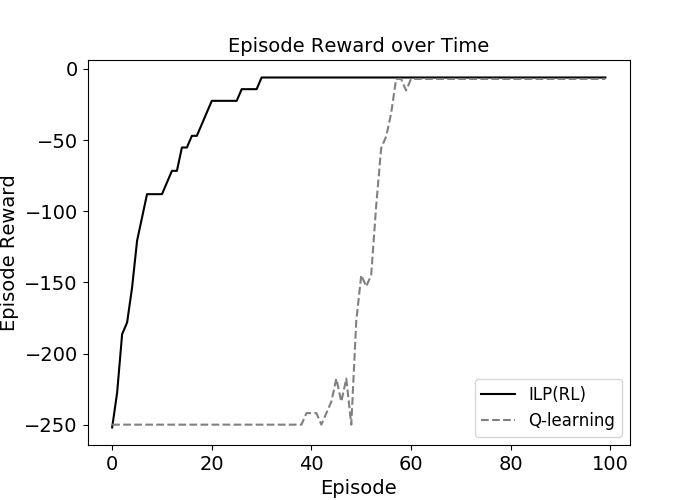
\includegraphics[width=1.0\textwidth]{./figures/experiment1_test}
\caption{Experiment 1 results of test performance}
\label{experiment1_test}
\end{figure}

Figure \ref{experiment1_training} shows the traning performance between ILP(RL) and Q-learning.
The convergence rate of ILP(RL) is faster than Q-learnig: ILP(RL) reaches the maximum reward between 40 and 50 episodes, whereas Q-learning reaches the same level at between 60 and 70 episodes.
This is because unlike Q-learning where the value function is updated with the rate of alpha, whereas ILP(RL) gradually builds the model of the environment and use the background knowledge to accurately plan.
This result is also consistent with the general notion that model-based learnig (ILP(RL)) is more data-efficient than model-free learning (Q-learning).
The same trend is also shown in Figure \ref{experiment1_test}, where we measure only the performance of the policy without random exploration.

Overall this results shows that ILP(RL) converges to the optimal policy faster than benchmarks in a simple scenarios, achieving more data-efficient learning.


In addition to the data-efficient learning, what the agent has learnt with ILP(RL) is expressive.
Learnt hypotheses are shown in \ref{experiment1_hypothesis}, which is the rule of the game and easy to understand for human users.
Since the learnt hypothesis is a general concept, which can be used in a different environmet.
This transfer learning capability is also described in Experiement 3 and 4.

\begin{equation}
\begin{split}
&\textsf{state\_after(V1) :- adjacent(right, V0, V1), state\_before(V1), action(right), wall(V0).}\\
&\textsf{state\_after(V0) :- adjacent(right, V0, V1), state\_before(V0), action(left), wall(V1).}\\
&\textsf{state\_after(V1) :- adjacent(down, V0, V1), state\_before(V1), action(down), wall(V0).}\\
&\textsf{state\_after(V1) :- adjacent(up, V0, V1), state\_before(V1), action(up), wall(V0).}\\
&\textsf{state\_after(V0) :- adjacent(right, V0, V1), state\_before(V1), action(right), not wall(V0).}\\
&\textsf{state\_after(V0) :- adjacent(left, V0, V1), state\_before(V1), action(left), not wall(V0).}\\
&\textsf{state\_after(V0) :- adjacent(down, V0, V1), state\_before(V1), action(down), not wall(V0).}\\
&\textsf{state\_after(V0) :- adjacent(up, V0, V1), state\_before(V1), action(up), not wall(V0).}
\end{split}
\end{equation}
\label{experiment1_hypothesis}

In addition, we plot the learning convergence for ILASP at episode 0 in Figure \ref{experiment1_ilasp}, measured in terms of the number of hypothesis refinement to reach the final hypothesis as shown in \ref{experiment1_hypothesis}.
This shows that the agent quickly learns the hypothesis at the episode 0. The reason that the agent reaches the maximum reward at between 40 and 50 episodes, is mostly dependent on how quickly the agent finds the goal location,
which enables it to plan. Since our exploration strategy is expilon random choice, there is a promissing that a better exploration strategy further accelerates the learning process.

\begin{figure}[!htb]
\centering
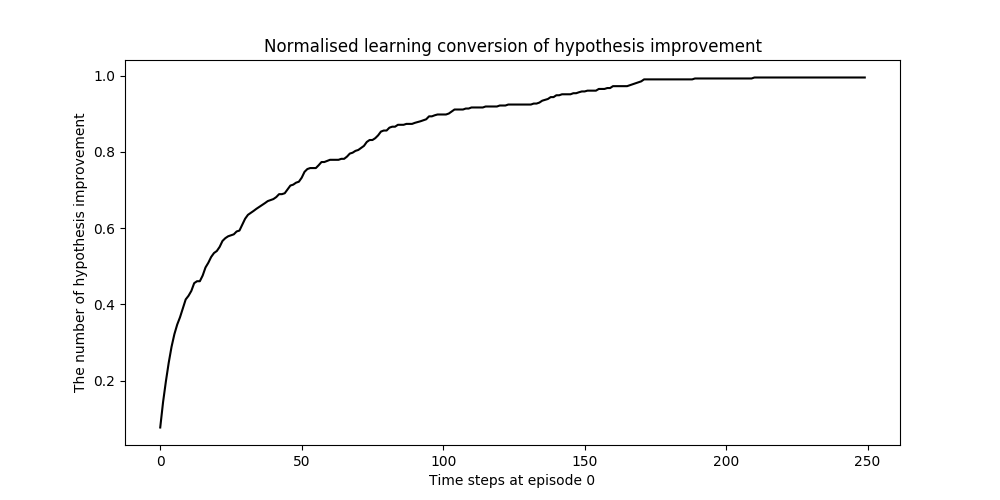
\includegraphics[width=1.0\textwidth]{./figures/experiment1_ilasp}
\caption{Learning convergence of hypothesis improvement by ILP(RL) (normalised)}
\label{experiment1_ilasp}
\end{figure}

\newpage
\subsection{Experiment2}
% The game is designed such that

\begin{figure}[!htb]
\centering
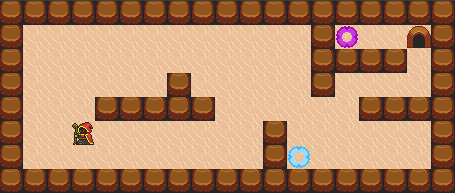
\includegraphics[width=0.5\textwidth]{./figures/experiment3}
\caption{Enviroment for experiment 2}
\label{experiment3}
\end{figure}

Experiment 2 was conducted to see if the agent find a optimal path of using a teleport. In the environment shown in Figure \ref{experiment3},
there are two ways to reach the goal: using a normal path to get the goal located on the top right corner, or using a telport.
The environment is designed such that using a teleport is a shorter path and therefore gives higher total reward.
Compared to Experiment 1, two extra search spaces and concepts are added as follow:
\begin{equation*}
\begin{split}
&\textsf{\#modeb(1, link\_start(var(cell)), (positive)).}\\
&\textsf{\#modeb(1, link\_dest(var(cell)), (positive)).}
\end{split}
\end{equation*}

Where teleport links are added to the environment. The teleport link is one-way: link\_start takes the agent to link\_dest, but link\_dest does not take the agent back to link\_start.
The allows ILASP to learn additional hypothesis.
The full learning task for this experiment is in Appendix XX.

Once the agent steps onto a state where link\_start is located, it gets two positive experiences.
In this game environment, the agent moves two cells in one time step instead of one cell per time step.

Also link\_start and link\_dest need to be stored in background knowledge rather than as contex examples,
because ILASP needs to learn different hypothesis for link and non-link case.
link locations need to be available for all positive examples so that ILASP correctly learn non-link, which is shown in Figure XX below.

\begin{figure}[!htb]
\centering
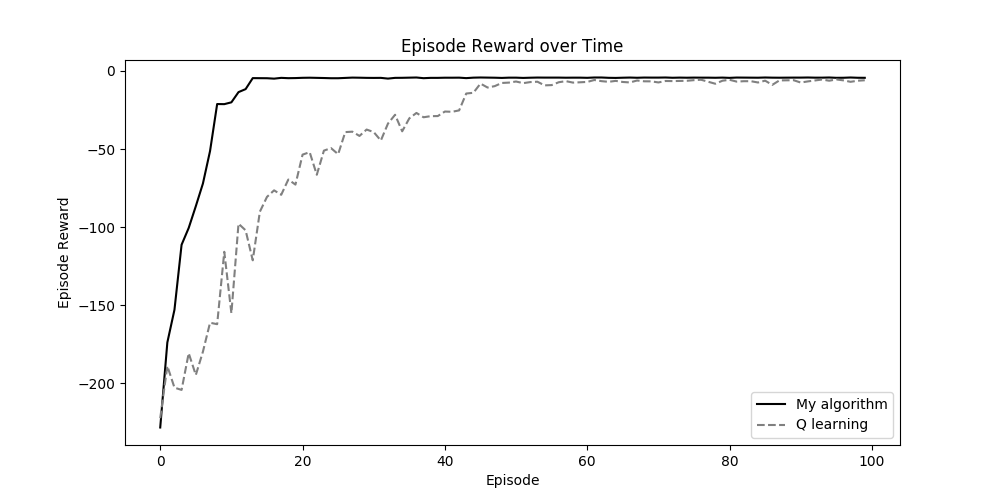
\includegraphics[width=1.0\textwidth]{./figures/experiment3_training}
\caption{Experiment 2 results of training performance}
\label{experiment3_training}
\end{figure}

The training performance shown in XX, which converges faster than XX.

\begin{figure}[!htb]
\centering
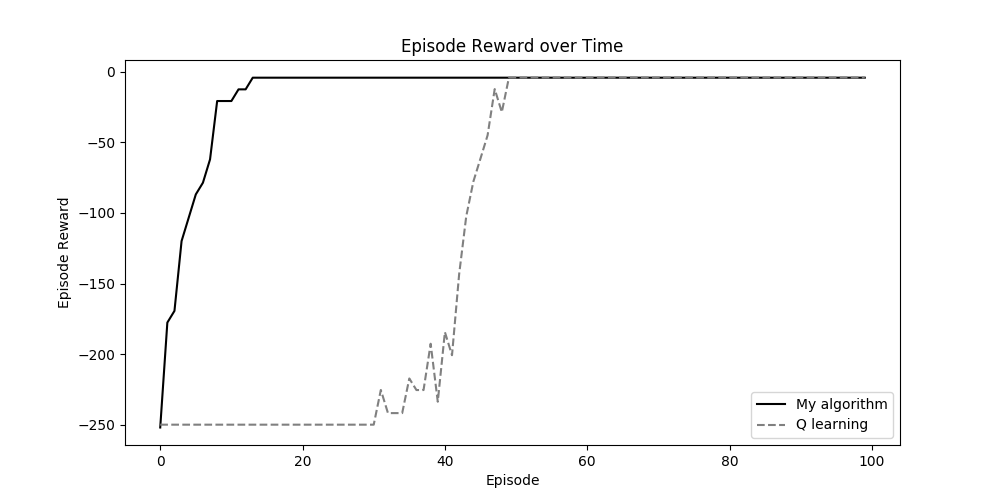
\includegraphics[width=1.0\textwidth]{./figures/experiment3_test}
\caption{Experiment 2 results of test performance}
\label{experiment3_test}
\end{figure}

\begin{equation}
\begin{split}
&\textsf{state\_after(V1) :- link\_dest(V1).}\\
&\textsf{state\_after(V0) :- link\_dest(V0), state\_before(V0), action(right).}\\
&\textsf{state\_after(V1) :- adjacent(left, V0, V1), state\_before(V0), action(right), not wall(V1).}\\
&\textsf{state\_after(V0) :- adjacent(left, V0, V1), state\_before(V1), action(left), not wall(V0).}\\
&\textsf{state\_after(V1) :- adjacent(up, V0, V1), state\_before(V0), action(down), not wall(V1).}\\
&\textsf{state\_after(V0) :- adjacent(up, V0, V1), state\_before(V1), action(up), not wall(V0).}\\
&\textsf{state\_after(V1) :- adjacent(left, V0, V1), state\_before(V1), action(left), wall(V0).}\\
&\textsf{state\_after(V1) :- adjacent(down, V0, V1), state\_before(V1), action(down), wall(V0).}\\
&\textsf{state\_after(V1) :- adjacent(up, V0, V1), state\_before(V1), action(up), wall(V0).}
\end{split}
\label{experiment2_ilasp_imcomplete}
\end{equation}

To highlight the learning the new concept of teleport link, Figure \ref{experiment2_ilasp_imcomplete} is an intermediate incomplete hypothesis learnt by ILASP.
These hypotheses are generated just after the agent steps onto the link. However, the first hypothesis says
when link\_dest is available state\_after is true. Since link\_dest is available in background knowledge rather than context,
when solving for answer sets to generate a plan, it generates incorrect state\_after at every time step.
However, as shown in Algorithms XX, these generated state\_after are all incorrect and therefore will be added to exclusions of the next positive examples.
These exclusions will later refines hypotheses and results in Figure \ref{experiment2_ilasp_complete}, the final complete hypotheses.

Learnt hypotheses are as follow:
\begin{equation}
\begin{split}
&\textsf{state\_after(V1) :- link\_start(V0), link\_dest(V1), state\_before(V0).}\\
&\textsf{state\_after(V0) :- link\_dest(V0), state\_before(V0), action(right).}\\
&\textsf{state\_after(V1) :- adjacent(left, V0, V1), state\_before(V0), action(right), not wall(V1).}\\
&\textsf{state\_after(V0) :- adjacent(left, V0, V1), state\_before(V1), action(left), not wall(V0).}\\
&\textsf{state\_after(V1) :- adjacent(up, V0, V1), state\_before(V0), action(down), not wall(V1).}\\
&\textsf{state\_after(V0) :- adjacent(up, V0, V1), state\_before(V1), action(up), not wall(V0).}\\
&\textsf{state\_after(V1) :- adjacent(left, V0, V1), state\_before(V1), action(left), wall(V0).}\\
&\textsf{state\_after(V1) :- adjacent(down, V0, V1), state\_before(V1), action(down), wall(V0).}\\
&\textsf{state\_after(V1) :- adjacent(up, V0, V1), state\_before(V1), action(up), wall(V0).}
\end{split}
\label{experiment2_ilasp_complete}
\end{equation}

Compared the Experiment 1, there are two new hypotheses due to the presence of the teleport links.
These learnt hypotheses are also applicables to an environment where there is no link, such as a game in experiment 1.
In this case, the first two hypotheses in Figure XX are never be used since the body predicates relating to link\_start(V0), link\_dest(V1) are never be satisfied.

\begin{figure}[!htb]
\centering
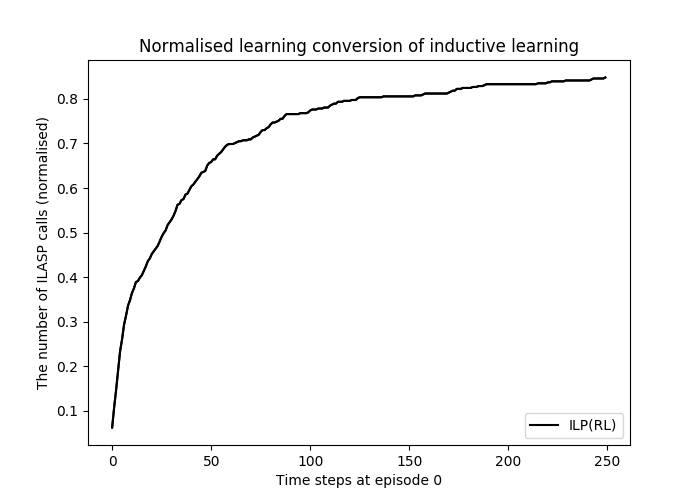
\includegraphics[width=1.0\textwidth]{./figures/experiment2_ilasp}
\caption{Learning convergence of hypothesis improvement by ILP(RL) (normalised)}
\label{experiment1_test}
\end{figure}

\newpage

\subsection{Experiment3}

\begin{figure}[!htb]
\centerline{
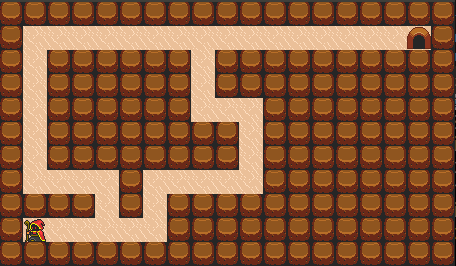
\includegraphics[width=0.5\textwidth]{./figures/experiment4_before}
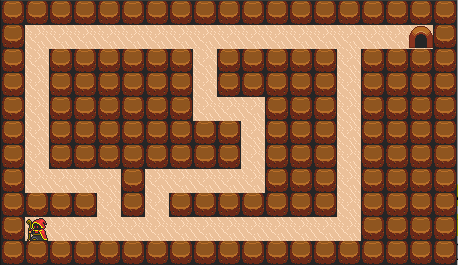
\includegraphics[width=0.5\textwidth]{./figures/experiment4_after}
}
\caption{Environment used before (left) and after (right) transfer learning}
\label{experiment3}
\end{figure}

In Experiment 3, we investigated the potentials of transfer learning betweeen similar environments.
We trained the agent using the environment on the left in Figure \ref{experiment4}, and transfer the learnt hypothesis as well as positive examples to a new environment.
The learnt hypothesis is valid move of the game and a general concept that is applicable to any similar games. Positive examples are also transferred since
if there is a new concept that the agent needs to learn in a new environment, the agent needs to refine the hypothesis by running ILASP, thus the all the positice examples
are also transferred as well as hypotheses. Background knowledge are not transferred since these information are different in a new environment.
The agent starts with an empty background knowledge in the new environment and gradually collects them
as it explore the environment. The goal position is the same as in the first game and we assume that the transferred agent already knows the goal location, but the routes to the goal may be different.
While this is a limited transfer learning since the goal position is known in advance, this is still a useful transfer in cases where the rest of the environment changes.
In this experiment, we compare the two learning performance: one with transfer learning and one without it.
The result is shown in Figure \ref{experiment3_training} and \ref{experiment3_test}.

These are the hypotheses we are transferring to a new environment.
Since the complete hypothesis is already known to the agent, it can do planning from the beginning.

\begin{equation}
\begin{split}
 &\textsf{state\_after(V0) :- adjacent(right, V0, V1), state\_before(V1), action(right), not wall(V0).}\\
 &\textsf{state\_after(V0) :- adjacent(left, V0, V1), state\_before(V1), action(left), not wall(V0).}\\
 &\textsf{state\_after(V1) :- adjacent(down, V0, V1), state\_before(V0), action(up), not wall(V1).}\\
 &\textsf{state\_after(V0) :- adjacent(down, V0, V1), state\_before(V1), action(down), not wall(V0).}\\
 &\textsf{state\_after(V1) :- adjacent(right, V0, V1), state\_before(V1), action(right), wall(V0).}\\
 &\textsf{state\_after(V1) :- adjacent(left, V0, V1), state\_before(V1), action(left), wall(V0).}\\
 &\textsf{state\_after(V0) :- adjacent(up, V0, V1), state\_before(V0), action(down), wall(V1).}\\
 &\textsf{state\_after(V1) :- adjacent(up, V0, V1), state\_before(V1), action(up), wall(V0).}
\end{split}
\end{equation}

\begin{figure}[!htb]
\centering
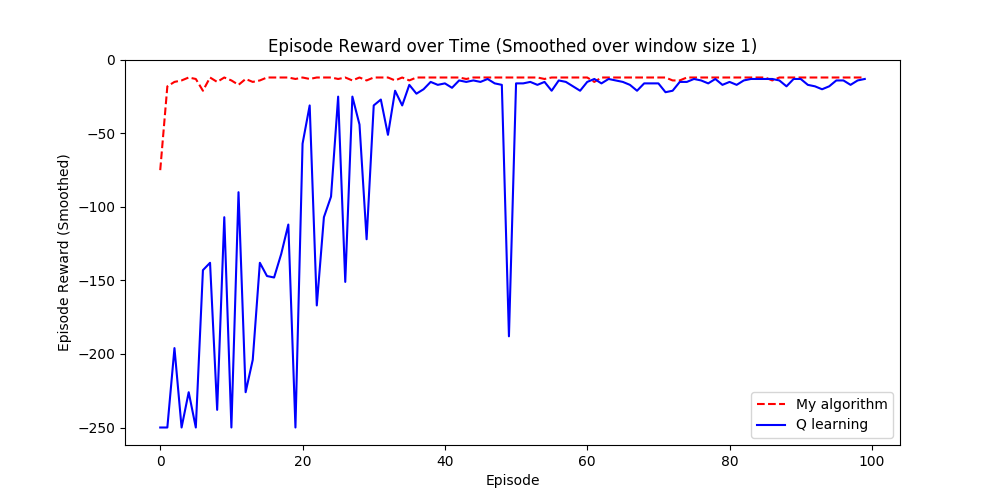
\includegraphics[width=1.0\textwidth]{./figures/experiment4_after_training}
\caption{Experiment 3 results of training performance with and without transfer learning}
\label{experiment3_training}
\end{figure}

\begin{figure}[!htb]
\centering
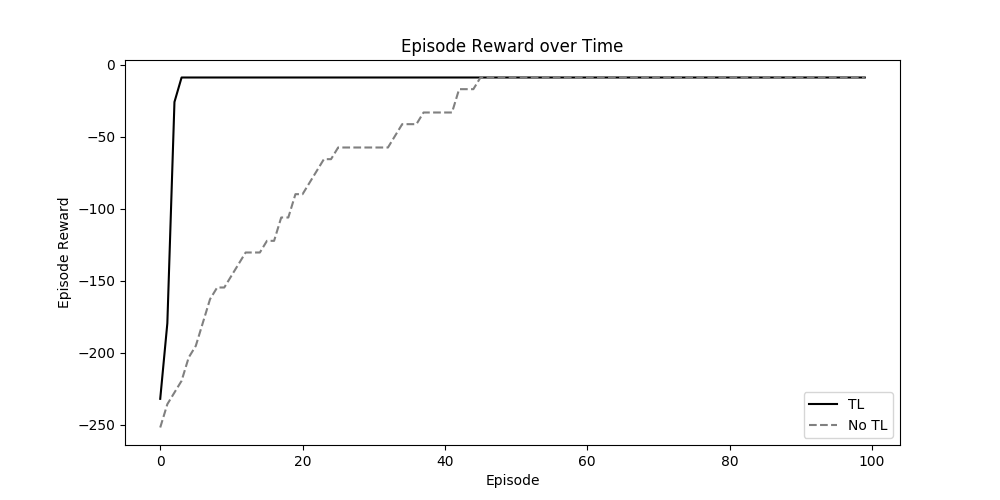
\includegraphics[width=1.0\textwidth]{./figures/experiment4_after_test}
\caption{Experiment 3 results of test performance with and without transfer learning}
\label{experiment3_test}
\end{figure}

\subsection{Experiment4}

\begin{figure}[!htb]
\centerline{
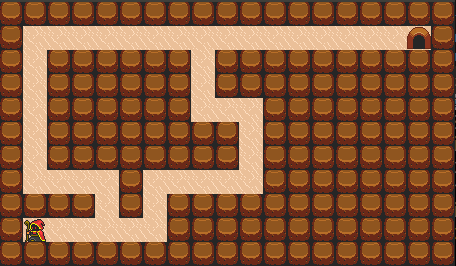
\includegraphics[width=0.5\textwidth]{./figures/experiment4_before}
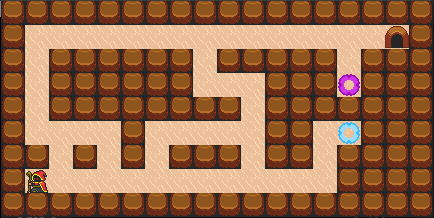
\includegraphics[width=0.5\textwidth]{./figures/experiment5_after}}
\caption{Environment used before (left) and after (right) transfer learning}
\label{experiment5}
\end{figure}

Finally the hypothesis is transferred to a new environment where there is a new concept that did not exist in the first environment
and therefore the agent needs to learn it after the hypothesis is transferred.

\begin{figure}[!htb]
\centering
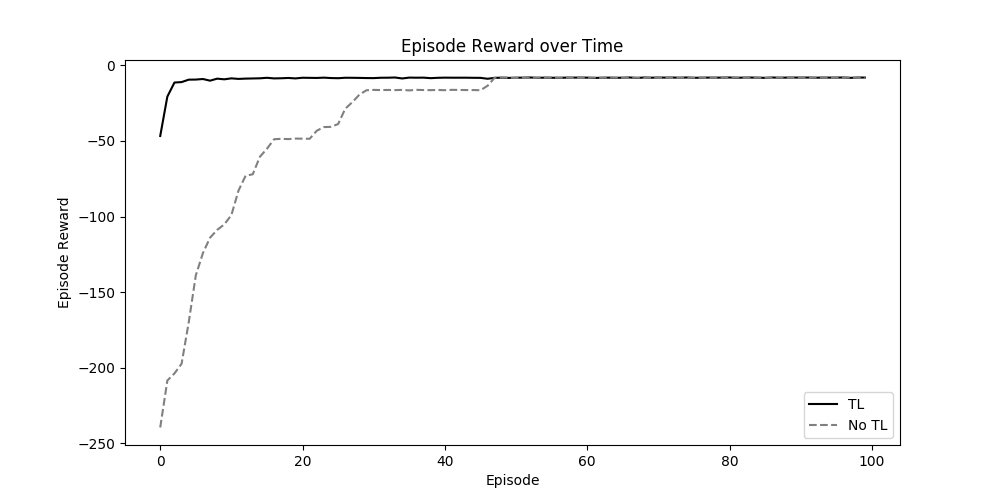
\includegraphics[width=1.0\textwidth]{./figures/experiment5_training}
\caption{Comparison of training performance between ILP(RL) with and without transfer learning}
\label{experiment5_training}
\end{figure}

\begin{figure}[!htb]
\centering
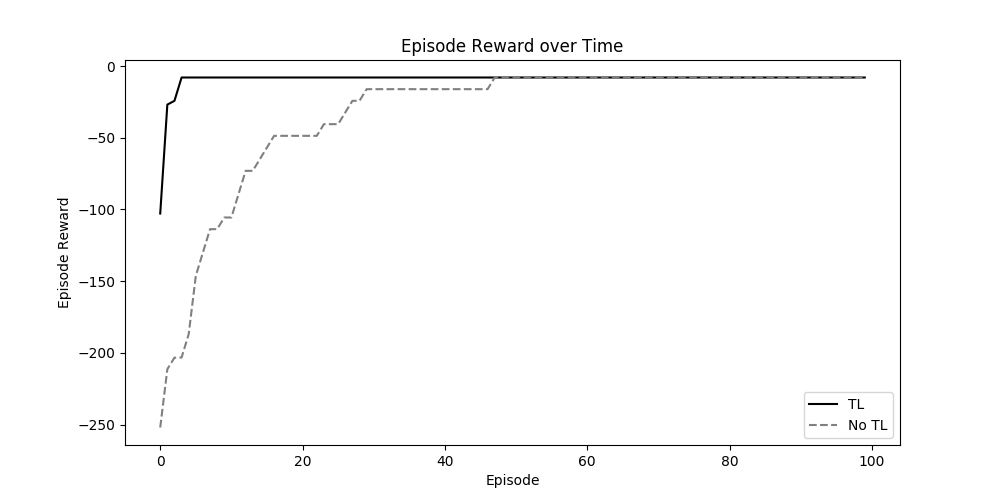
\includegraphics[width=1.0\textwidth]{./figures/experiment5_test}
\caption{Comparison of test performance between ILP(RL) with and without transfer learning}
\label{experiment5_test}
\end{figure}

\begin{equation}
\begin{split}
&\textsf{state\_after(V1) :- link\_start(V0), link\_dest(V1), state\_before(V0).}\\
&\textsf{state\_after(V1) :- adjacent(left, V0, V1), state\_before(V0), action(right), not wall(V1).}\\
&\textsf{state\_after(V0) :- adjacent(left, V0, V1), state\_before(V1), action(left), not wall(V0).}\\
&\textsf{state\_after(V1) :- adjacent(up, V0, V1), state\_before(V0), action(down), not wall(V1).}\\
&\textsf{state\_after(V0) :- adjacent(up, V0, V1), state\_before(V1), action(up), not wall(V0).}\\
&\textsf{state\_after(V0) :- adjacent(left, V0, V1), state\_before(V0), action(right), wall(V1).}\\
&\textsf{state\_after(V1) :- adjacent(left, V0, V1), state\_before(V1), action(left), wall(V0).}\\
&\textsf{state\_after(V0) :- adjacent(up, V0, V1), state\_before(V0), action(down), wall(V1).}\\
&\textsf{state\_after(V1) :- adjacent(up, V0, V1), state\_before(V1), action(up), wall(V0).}
\end{split}
\label{experiment4_ilasp}
\end{equation}
